% https://en.wikipedia.org/wiki/Capacitor#DC_circuits

\documentclass{article} %minimal is cool too

\usepackage{graphicx}
\usepackage[outdir=./]{epstopdf} % for including .esp

\usepackage{empheq} % for equation highlighting

\usepackage{amsmath}

\begin{document}

\title{Derivation of the Normal Vector to a 2D Electric Potential Surface}
\author{Joe Iddon}
\date{March 20, 2020}
\maketitle

The electric potential field is three dimensional and scalar. A two dimensional electric potential field, concerned only with charges in the same XY-plane, can be visualised by a surface, $\textbf{S}$. The Z-dimension of the surface is equal to the electric potential at the corresponding XY-coordinate.

%https://en.wikipedia.org/wiki/Surface_(mathematics)#Graph_of_a_bivariate_function

The surface can be parameterised by a bivariate function $z = f(x,y)$. This function, $f(x,y)$, must calculate the electric potential at the point $(x,y)$ given the locations and charge of all known charges.

The electric potential at position $(x,y)$ due to charge $i$ is given by

$$V = -k\frac{q_i}{\sqrt{(x-x_i)^2 + (y-y_i)^2}}$$

where the charge has location $(x_i, y_i)$ and charge $q_i$.

Due to the principle of super position, the total electric potential can be calculated by summing over all charges.

$$f(x,y) = -k\sum_{i}\frac{q_i}{\sqrt{(x-x_i)^2 + (y-y_i)^2}}$$

This describes $\textbf{S}$, allowing it to be easily plotted using computer software by iterating over a grid of $(x,y)$ locations and generating the height of the surface using this formula. The surface can then be triangulated and rendered. This can be seen in Figure~\ref{fig:no-shading}.

\begin{figure}
\label{fig:no-shading}
\includegraphics[width=\linewidth]{no_shading.png}
\caption{The electric potential visualisation without shading.}
\end{figure}

This s

\begin{figure}
\label{fig:shading}
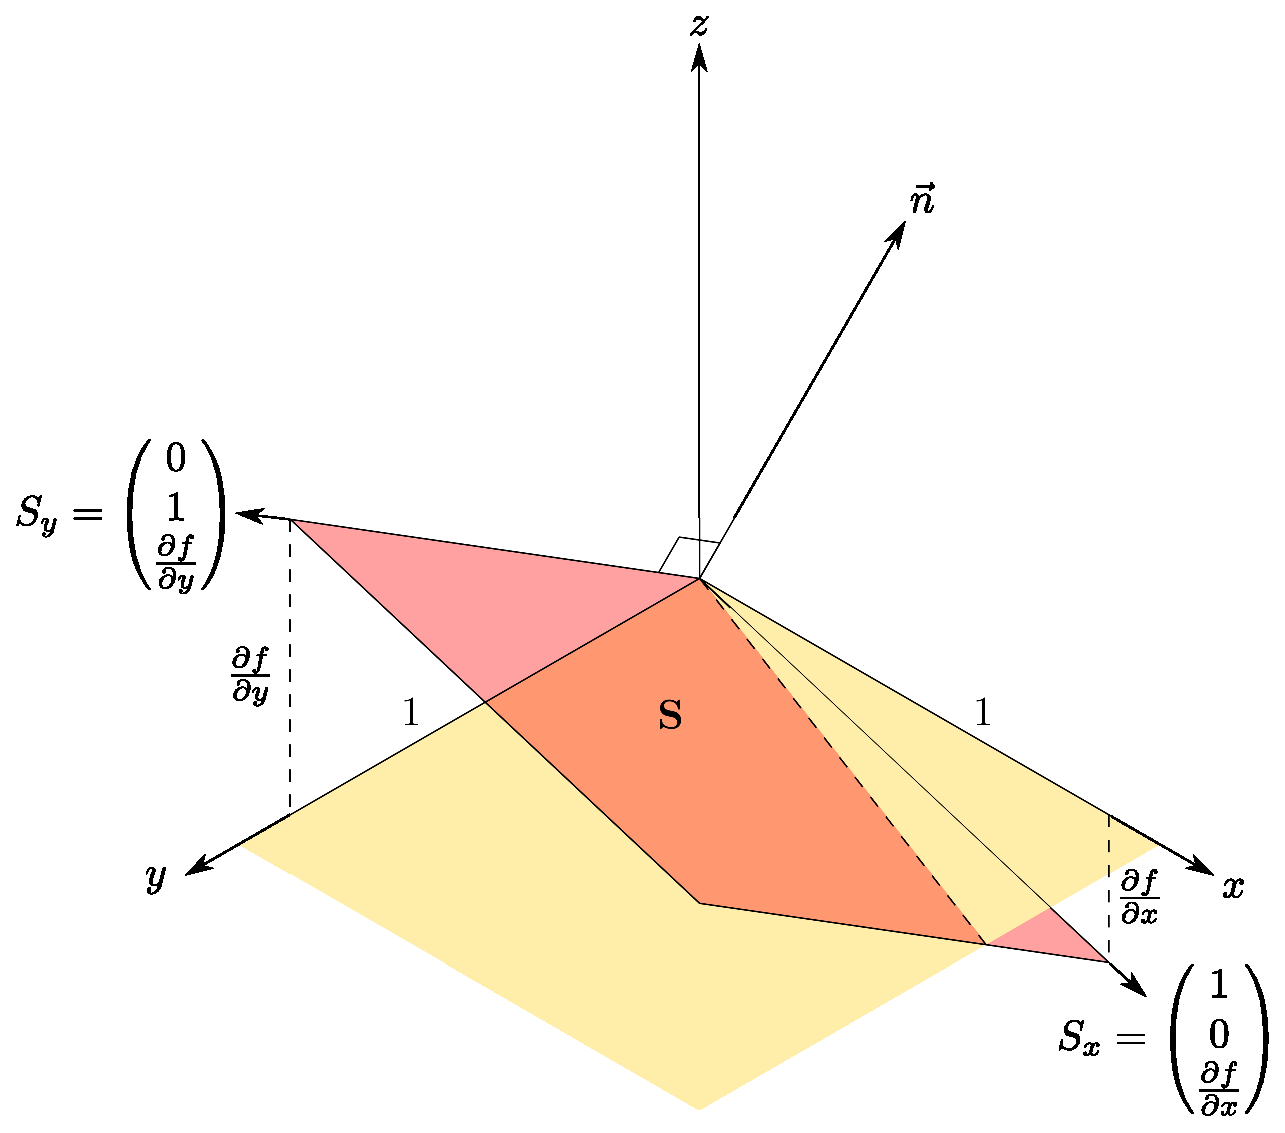
\includegraphics[width=\linewidth]{diagram.eps}
\caption{The electric potential visualisation with shading.}
\end{figure}


\begin{figure}
\label{fig:shading}
\includegraphics[width=\linewidth]{shading.png}
\caption{The electric potential visualisation with shading.}
\end{figure}

\end{document}